\documentclass[english]{article}
\usepackage[T1]{fontenc}
\usepackage[latin9]{inputenc}
\usepackage{hyperref}
\usepackage{graphicx}

\usepackage{parskip}
%\usepackage{babel}
\begin{document}

\title{Apache Spark Quick Guide \\
Python}


\author{Joshua Jansen Van Vueren}

\maketitle

\section*{Introduction}
This document seeks to outline and describe the programming model utilised by Apache Spark, and compare utility to other frameworks.
\\\\
"Apache Spark is a fast and general-purpose cluster computing system." 
\\
"Apache Spark lets you use clusters of tens, hundreds, or thousands of servers to run simulations in a way that is intuitive and scales to meet your needs."
\\
"Overall, Spark has been a flexible, robust and scalable data processing engine... Spark Streaming provides efficient fault-tolerant stateful stream processing. It provides high throughput and good integration with data stores like Cassandra, Kafka, Hadoop etc."
\section{Terminology}
\begin{itemize}
\item \textbf{Resilient Distributed Datasets - RDD:} Fault-tolerant collection of elements that can be operated on in parallel. Optimized for parallel processing.
\item \textbf{Dataset:} Distributed collection of data, newer programming interface, better performance over RDD's.
\item \textbf{DataFrame:} Dataset organized into named columns, conceptually equivalent to a relational DB table (supported in Scala,Java,Python,R).
\item \textbf{DStreams:} Sequence of RDD's as defined by user based of time intervals (micro-batching).
\item \textbf{Parallelization:} Members from collection are copied to form a distributed dataset, to be operated on in parallel. Slicing the data into a number of partitions to be used in the cluster.
\item \textbf{External Datasets:} Spark can create distributed datasets from any storage source supported by Hadoop.
\item \textbf{Cluster:} Groups of Compute Engine VM's with master and worker VM's.
\item \textbf{Cloud Dataproc:} Google Cloud Dataproc lets you provision Apache Hadoop clusters and connect to underlying analytic data stores. "Can provision capacity on demand and pay for it by the minute". Spark jobs can be submitted and run on Dataproc. 
\end{itemize}
\section{Systems}
\subsection{Beam}
\begin{itemize}
\item Beam provides the ability to utilise multiple different runners, these runners are compared through a capability matrix - \href{https://beam.apache.org/documentation/runners/capability-matrix/}{available here}. From the matrix it is clear that all areas considered in data processing the number functionalities provided by Dataflow outweigh Spark.
\item So one can utilise Spark to run Apache Beam pipelines, but Spark can also be run independently.
\end{itemize}
\subsection{Spark}
\begin{itemize}
\item Memory Intensive
\item Streaming builds micro-batches (micro-batch size is a pre-set, fixed, time interval), processed by Spark engine, outputting processed data. Not per record stream.
\item Data is structured in RDD's which is analogous to Beam's PCollection.
\item Utility being a all-in-one solution for all processing needs.
\item Can be run locally using servers or online utilising BigQuery, DataProc etc.
\item Streaming Inputs: Kafka, Flume, Kinesis, or TCP sockets
\item MLib can be applied to data-streams. There are streaming ML algorithms which learn from streaming data and are applied to streaming data, and there are models which can be learned off historical data (offline) and then applied to streaming data.
\item Streaming Outputs: Filesystems, databases, and live dashboards
\item It seems that scaling the jobs is handled by Spark, however it may be required to allocate more resources should the jobs require it.
\end{itemize}
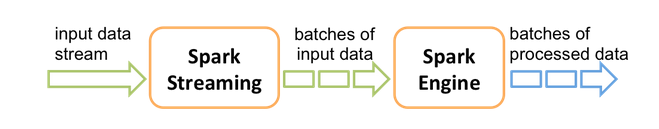
\includegraphics[scale=0.5]{spark_streaming_model.png}
\\\\
\subsubsection{Spark Use Cases}
\begin{itemize}
\item Streaming Data
	\begin{itemize}
		\item Streaming Extract, Transform, Load
		\item Data Enrichment
		\item Trigger Event Detection
		\item Complex Session Analysis - session activity easy to group and analyse
	\end{itemize}
\item ML
\item Fog Computing
\end{itemize}
\textbf{Industry Use Cases:}
\begin{itemize}
\item Booking.com utilises spark for online ML features for real-time prediction of behaviour and preference of users.
\item \href{https://medium.com/walmartlabs/how-we-built-a-data-pipeline-with-lambda-architecture-using-spark-spark-streaming-9d3b4b4555d3}{Walmart Labs Pipeline using Spark Streaming}
\end{itemize}
\subsubsection{Utilities:}
\begin{itemize}
\item Able to read from and write to BigQuery, \href{https://cloud.google.com/dataproc/docs/tutorials/bigquery-connector-spark-example}{code here}.
\item Can run ML algorithms from BigQuery data, \href{https://cloud.google.com/dataproc/docs/tutorials/bigquery-sparkml#spark-ml-tutorial_subset-python}{code here}.
\item Processes data from Pub/Sub using Dataproc and outputs to Datastore, \href{https://cloud.google.com/solutions/using-apache-spark-dstreams-with-dataproc-and-pubsub#whats-next}{code here}
\item PySpark does have some streaming capabilities, but is limited in connectors, connectors like Kafka are supported; \href{https://spark.apache.org/docs/1.5.2/api/python/pyspark.streaming.html}{Py Spark Streaming Library}. I have yet to see a streaming example of PySpark that reads from and writes to any cloud storage, they all seem to implemented in a batch mode.
\end{itemize}
\subsubsection{Libs:}
\begin{itemize}
\item \textbf{MLib} \url{https://spark.apache.org/docs/2.0.0/ml-guide.html}
\end{itemize}
\subsubsection{RDD Operations}
\begin{itemize}
\item \textbf{Transformations:} Create new dataset from an existing one
\item \textbf{Actions:} Return a value to the driver program after running a computation on the dataset.
\item \textbf{Note:} All transformations are lazy, therefore they do not compute all results immediately, only when required - by an action. One would need to run a \verb"collect()" or some other action.
\item \textbf{Models:} ML models can be run on data through the spark structure, \href{https://github.com/apache/spark/blob/master/examples/src/main/python/kmeans.py}{example here}
\end{itemize}
\subsection{Kafka}
\begin{itemize}
\item Data Pipeline
\item Record-at-a-time processing
\end{itemize}
\subsection{Hive}
\begin{itemize}
\item Horizontally scalable
\item SQL Interface, operating on Hadoop
\item Built for data warehousing operations
\end{itemize}
\subsection{Comparisons}
\textbf{Spark vs Beam:} Apache Beam can be classified as a tool in the "Workflow Manager" category, while Apache Spark is grouped under "Big Data Tools" \footnote{https://stackshare.io/stackups/apache-beam-vs-spark}.\\\\
\textbf{Spark vs Hadoop:} Hadoop is more focused towards batching, and spark towards streaming. Spark utilises HDFS for its file structuring. Spark was built over the Hadoop framework to achieve faster data processing in both batch and streaming applications, at the cost of being more memory intensive.
\section{Other Documentation and Links}
\begin{itemize}
\item \href{https://cloud.google.com/dataproc/docs/tutorials/gcs-connector-spark-tutorial}{Google Cloud Storage Connector with Apache Spark}
\item \href{https://www.qubole.com/blog/apache-spark-use-cases/}{Apache Spark Use Cases}
\item \href{https://cloud.google.com/docs/authentication/getting-started}{Google Cloud Console Authentication Setup}
\item \href{https://jaceklaskowski.gitbooks.io/mastering-apache-spark/spark-rdd-caching.html}{Caching in Spark}
\item \href{https://medium.com/capital-one-tech/filtering-vs-enriching-data-in-apache-spark-e44108c3a372}{Filtering Vs Enriching Data in Apache Spark}; interesting use case.
\end{itemize}
\section{Where to Go From Here}
\begin{itemize}
\item I would shift over to implementing Spark in Scala. It seems required if one would like to access the full capabilities of the system. There are numerous examples of streaming pipeline examples written in Scala.
\item It is my intuition that there may be a way around the constraint of only batch implementations in PySpark. It would seem that \href{https://cloud.google.com/dataproc/docs/concepts/workflows/overview}{WorkFlows} in DataProc would have the ability to schedule jobs, and the BigQuery connector provided one could implement a windowing query. Alternatively a \href{https://stackoverflow.com/questions/30375571/running-scheduled-spark-job}{cron job} could do the trick.
\item The new graph library in Spark could be of some utility, \href{https://spark.apache.org/docs/latest/graphx-programming-guide.html}{available here}.
\end{itemize}
\end{document}
